\documentclass[DaoFP]{subfiles}
\begin{document}
\setcounter{chapter}{13}

\chapter{Monads and Ajdunctions}

\section{String Diagrams}

A line partitions a plane. We can think of it as either dividing a plane or as connecting two half-planes.

A dot partitions a line. We can think of it as either separating two half-lines or as joining them together.

This is a diagram in which two categories are represented as dots, two functors as arrows, and a natural transformation as a double arrow.

\[
\begin{tikzpicture}[column sep=huge]
\def \xa{-1.2};
\def \xb{0};
\def \xc{1.2};
\def \ya{-1};
\def \yb{0};
\def \yc{1};

\node(c) at (\xa, \yb) {};
\node[left] at (c) {$\mathcal{C}$};
\filldraw[black] (c) circle (1 pt);
\node(d) at (\xc, \yb) {};
\node[right] at (d) {$\mathcal{D}$};
\filldraw[black] (d) circle (1 pt);

\draw [->] (c) to [out=60,in=120] node[midway, above]{$G$}(d);
\draw [->] (c) to [out=-60,in=-120] node[midway, below]{$F$}(d);

\node(mup) at (\xb, \yc -0.5) {};
\node(mdn) at (\xb, \ya + 0.5) {};
\draw[->, -{Implies}, double, double distance=2pt] (mdn) -- node[midway, left]{$\alpha$} (mup);
\end{tikzpicture}
\]

But the same idea can be represented by drawing categories as areas of a plane, functors that connect them as lines between areas, and natural transformations as dots that partition line segments. 

The idea is that a functor always goes between a pair of categories, therefore it can be drawn as a boundary between them. A natural transformation always goes between a pair of functors, therefore it can be drawn as a dot joining two halves of a line.

\[
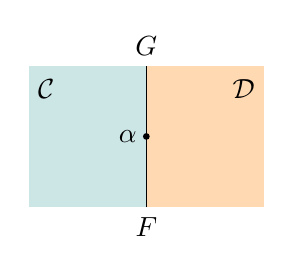
\begin{tikzpicture}
\def\x{0};
\def\xl{-1.5};
\def\xr{1.5};


\def \ya{0.8};
\def \yb{1.7};
\def \yc{2.6};
\def \yt {2.3};

\filldraw[fill=blue!50!green!20, draw=white] (\xl, \ya) rectangle (\x, \yc);
\filldraw[fill=orange!30, draw=white] (\x, \ya) rectangle (\xr, \yc);

\node[below] (a) at (\x, \ya) {$F$};
\node(b) at (\x, \yb) {};
\node [above] (c) at (\x, \yc) {$G$};

\node(l)[right] at (\xl, \yt) {$\mathcal{C}$};
\node(r)[left] at (\xr, \yt) {$\mathcal{D}$};


\filldraw[black] (b) circle (1 pt);
\node [left] at (b) {$\alpha$};

\draw (a)  -- (c);

\end{tikzpicture}
\]

This is an example of a \emph{string diagram}. You read such a digram bottom-up, left-to-right (think of the $(x, y)$ system of coordinates). 

The bottom of this diagram shows a functor $F$ that goes from $\mathcal{C}$ to $\mathcal{D}$. The top of the diagram shows a functor $G$ that goes between the same two categories. The transition happens in the middle, where a natural transformation $\alpha$ maps $F$ to $G$.

So far it doesn't seem like we gain a lot by using this new visual representation. But let's apply it to something more interesting: vertical composition of natural transformations:
\[
\begin{tikzcd}[column sep=huge]
\mathcal{C}
  \arrow[bend left=60]{rr}[name=U, label=above:$H$]{}
  \arrow[]{rr}[name=M, label={[xshift=15pt, yshift=-5pt]:$G$}]{} 
  \arrow[bend right=60]{rr}[name=D, label=below:$F$]{} 
 &&
\mathcal{D}
  \arrow[shorten <=8pt, shorten >=8pt,Leftarrow, to path={(U) -- node[label=left:$\beta$] {} (M)}]{}
  \arrow[shorten <=8pt, shorten >=8pt,Leftarrow, to path={(M) -- node[label=left:$\alpha$] {} (D)}]{}
\end{tikzcd}
\]

The corresponding string diagram shows the two categories and three functors between them joined by two natural transformations.
\[
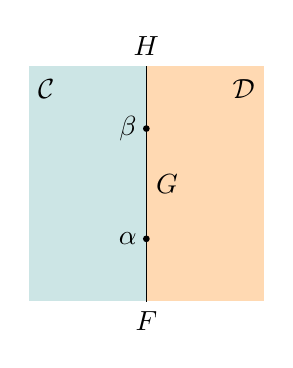
\begin{tikzpicture}
\def\x{0};
\def\xl{-1.5};
\def\xr{1.5};


\def \ya{0};
\def \yb{0.8};
\def \ybb{2.2};
\def \yc{3};
\def \yt {2.7};
\def \ymid {1.5}

\filldraw[fill=blue!50!green!20, draw=white] (\xl, \ya) rectangle (\x, \yc);
\filldraw[fill=orange!30, draw=white] (\x, \ya) rectangle (\xr, \yc);

\node[below] (a) at (\x, \ya) {$F$};
\node(b) at (\x, \yb) {};
\node(bb) at (\x, \ybb) {};
\node [above] (c) at (\x, \yc) {$H$};
\node(m)[right] at (\x, \ymid) {$G$};

\node(l)[right] at (\xl, \yt) {$\mathcal{C}$};
\node(r)[left] at (\xr, \yt) {$\mathcal{D}$};

\filldraw[black] (b) circle (1 pt);
\node [left] at (b) {$\alpha$};
\filldraw[black] (bb) circle (1 pt);
\node [left] at (bb) {$\beta$};

\draw (a)  -- (c);

\end{tikzpicture}
\]
As you can see, you can reconstruct the original diagram from the string diagram by scanning it bottom-to-top.

Let's continue with the horizontal composition of natural transformations:
\[
\begin{tikzcd}[column sep=huge]
\mathcal{C}
  \arrow[bend left=50]{r}[name=U, label=above:$F'$]{}
  \arrow[bend right=50]{r}[name=D, label=below:$F$]{} 
 &
\mathcal{D}
  \arrow[bend left=50]{r}[name=U1, label=above:$G'$]{}
  \arrow[bend right=50]{r}[name=D1, label=below:$G$]{} 
 &
\mathcal{E}
  \arrow[shorten <=10pt,shorten >=10pt,Leftarrow,to path={(U) -- node[label=left:$\alpha$] {} (D)}]{}
  \arrow[shorten <=10pt,shorten >=10pt,Leftarrow,to path={(U1) -- node[label=left:$\beta$] {} (D1)}]{}
\end{tikzcd}
\]
This time we have three categories, so we'll have three areas. 

The bottom of the string diagram corresponds to the composition of functors $G \circ F$ (in this order). The top corresponds to $G' \circ F'$. One natural transformation, $\alpha$, connects $F$ to $F'$; the other, $\beta$, connects $G$ to $G'$.
\[
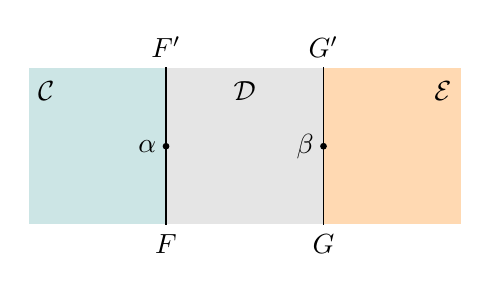
\begin{tikzpicture}
\def\xl{-2.75};
\def\xa{-1};
\def\xc{0}
\def\xb{1};
\def\xr{2.75};


\def \ya{0};
\def \yb{1};
\def \yc{2};
\def \yt {1.7};

\filldraw[fill=blue!50!green!20, draw=white] (\xl, \ya) rectangle (\xa, \yc);
\filldraw[fill=black!10!white, draw=white] (\xa, \ya) rectangle (\xb, \yc);
\filldraw[fill=orange!30, draw=white] (\xb, \ya) rectangle (\xr, \yc);

\node[below] (a) at (\xa, \ya) {$F$};
\node(b) at (\xa, \yb) {};
\node [above] (c) at (\xa, \yc) {$F'$};

\node[below] (d) at (\xb, \ya) {$G$};
\node(e) at (\xb, \yb) {};
\node [above] (f) at (\xb, \yc) {$G'$};

\node(l)[right] at (\xl, \yt) {$\mathcal{C}$};
\node(r) at (\xc, \yt) {$\mathcal{D}$};
\node(r)[left] at (\xr, \yt) {$\mathcal{E}$};


\filldraw[black] (b) circle (1 pt);
\node [left] at (b) {$\alpha$};
\filldraw[black] (e) circle (1 pt);
\node [left] at (e) {$\beta$};

\draw (a)  -- (c);
\draw (d)  -- (f);

\end{tikzpicture}
\]
Drawing two parallel vertical lines, in this new system, corresponds to functor composition. You can think of the composition of natural transformations as happening along the imaginary horizontal line in the middle of the diagram. But what if somebody was sloppy in drawing the diagram, and one of the dots was a little higher than the other? As it turns out, the exact positioning of the dots doesn't matter, due to the interchange law.

But first, let's illustrate whiskering: horizontal composition in which one of the natural transformation is the identity. We can draw it like this:

\[
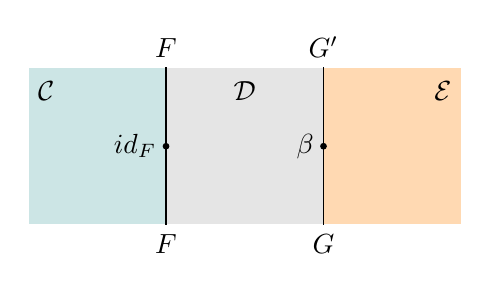
\begin{tikzpicture}
\def\xl{-2.75};
\def\xa{-1};
\def\xc{0}
\def\xb{1};
\def\xr{2.75};


\def \ya{0};
\def \yb{1};
\def \yc{2};
\def \yt {1.7};

\filldraw[fill=blue!50!green!20, draw=white] (\xl, \ya) rectangle (\xa, \yc);
\filldraw[fill=black!10!white, draw=white] (\xa, \ya) rectangle (\xb, \yc);
\filldraw[fill=orange!30, draw=white] (\xb, \ya) rectangle (\xr, \yc);

\node[below] (a) at (\xa, \ya) {$F$};
\node(b) at (\xa, \yb) {};
\node [above] (c) at (\xa, \yc) {$F$};

\node[below] (d) at (\xb, \ya) {$G$};
\node(e) at (\xb, \yb) {};
\node [above] (f) at (\xb, \yc) {$G'$};

\node(l)[right] at (\xl, \yt) {$\mathcal{C}$};
\node(r) at (\xc, \yt) {$\mathcal{D}$};
\node(r)[left] at (\xr, \yt) {$\mathcal{E}$};


\filldraw[black] (b) circle (1 pt);
\node [left] at (b) {$id_F$};
\filldraw[black] (e) circle (1 pt);
\node [left] at (e) {$\beta$};

\draw (a)  -- (c);
\draw (d)  -- (f);

\end{tikzpicture}
\]
But, really, the identity can be inserted at any point on a vertical line, so we don't even have to draw it. The following diagram represents the whiskering of $\beta \circ F$.
\[
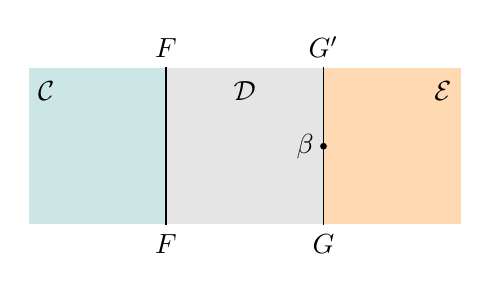
\begin{tikzpicture}
\def\xl{-2.75};
\def\xa{-1};
\def\xc{0}
\def\xb{1};
\def\xr{2.75};


\def \ya{0};
\def \yb{1};
\def \yc{2};
\def \yt {1.7};

\filldraw[fill=blue!50!green!20, draw=white] (\xl, \ya) rectangle (\xa, \yc);
\filldraw[fill=black!10!white, draw=white] (\xa, \ya) rectangle (\xb, \yc);
\filldraw[fill=orange!30, draw=white] (\xb, \ya) rectangle (\xr, \yc);

\node[below] (a) at (\xa, \ya) {$F$};
\node(b) at (\xa, \yb) {};
\node [above] (c) at (\xa, \yc) {$F$};

\node[below] (d) at (\xb, \ya) {$G$};
\node(e) at (\xb, \yb) {};
\node [above] (f) at (\xb, \yc) {$G'$};

\node(l)[right] at (\xl, \yt) {$\mathcal{C}$};
\node(r) at (\xc, \yt) {$\mathcal{D}$};
\node(r)[left] at (\xr, \yt) {$\mathcal{E}$};

\filldraw[black] (e) circle (1 pt);
\node [left] at (e) {$\beta$};

\draw (a)  -- (c);
\draw (d)  -- (f);

\end{tikzpicture}
\]
You can easily imagine the diagram for $\alpha \circ G$.

Here's the string diagram that corresponds to the interchange law:
\[
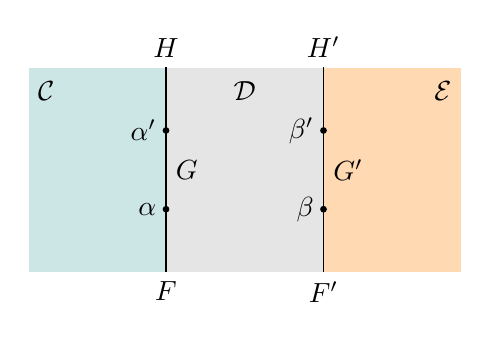
\begin{tikzpicture}
\def\xl{-2.75};
\def\xa{-1};
\def\xc{0}
\def\xb{1};
\def\xr{2.75};


\def \ya{0.2};
\def \yb{1};
\def \ybb{2}
\def \yc{2.8};
\def \yt {\yc -0.3};
\def \ymid {1.5}

\filldraw[fill=blue!50!green!20, draw=white] (\xl, \ya) rectangle (\xa, \yc);
\filldraw[fill=black!10!white, draw=white] (\xa, \ya) rectangle (\xb, \yc);
\filldraw[fill=orange!30, draw=white] (\xb, \ya) rectangle (\xr, \yc);

\node[below] (a) at (\xa, \ya) {$F$};
\node(b) at (\xa, \yb) {};
\node [above] (c) at (\xa, \yc) {$H$};
\node [right] (ml) at (\xa, \ymid) {$G$};

\node[below] (d) at (\xb, \ya) {$F'$};
\node(e) at (\xb, \yb) {};
\node [above] (f) at (\xb, \yc) {$H'$};
\node [right] (ml) at (\xb, \ymid) {$G'$};

\node(l)[right] at (\xl, \yt) {$\mathcal{C}$};
\node(r) at (\xc, \yt) {$\mathcal{D}$};
\node(r)[left] at (\xr, \yt) {$\mathcal{E}$};


\filldraw[black] (b) circle (1 pt);
\node [left] at (b) {$\alpha$};
\filldraw[black] (e) circle (1 pt);
\node [left] at (e) {$\beta$};

\node(bb) at (\xa, \ybb) {};
\node(ee) at (\xb, \ybb) {};

\filldraw[black] (bb) circle (1 pt);
\node [left] at (bb) {$\alpha'$};
\filldraw[black] (ee) circle (1 pt);
\node [left] at (ee) {$\beta'$};

\draw (a)  -- (c);
\draw (d)  -- (f);

\end{tikzpicture}
\]
This diagram is purposefully ambiguous. Are we supposed to first do vertical composition of natural transformations and then the horizontal one? Or should we compose $\beta \circ \alpha$ and $\beta' \circ \alpha'$ horizontally, and then compose the results vertically? The interchange law says that it doesn't matter: the result is the same. 

Now try to replace a pair of natural transformations in this diagram with identities. If you replace $\alpha'$ and $\beta'$, you get the horizontal composition of $\beta \circ \alpha$. If you replace $\alpha'$ and $\beta$, and rename $\beta'$ to $\beta$, you get the diagram in which $\alpha$ is shifted down with respect to $\beta$, and so on. The interchange law tells us that all these diagrams are equal. We are free to slide natural transformations like beads on a string.

\subsection{String diagrams for the monad}

A monad is defined as an endofunctor and two natural transformations, as illustrated by the following diagrams:
 
\[
\begin{tikzcd}[column sep=huge]
\mathcal{C}
  \arrow[bend left=50]{r}[name=U, label=above:$T$]{}
  \arrow[bend right=50]{r}[name=D, label=below:$\text{Id}$]{} 
 &
\mathcal{C}
  \arrow[shorten <=10pt,shorten >=10pt,Leftarrow,to path={(U) -- node[label=left:$\eta$] {} (D)}]{}
\end{tikzcd}
\hspace{20pt}
\begin{tikzcd}[column sep=huge]
\mathcal{C}
  \arrow[bend left=50]{r}[name=U, label=above:$T$]{}
  \arrow[bend right=50]{r}[name=D, label=below:$T \circ T$]{} 
 &
\mathcal{C}
  \arrow[shorten <=10pt,shorten >=10pt,Leftarrow,to path={(U) -- node[label=left:$\mu$] {} (D)}]{}
\end{tikzcd}
\]

Since we are dealing with just one category, when translating these diagrams to string diagrams, we can dispose of the naming (and shading) of categories, and just draw the strings alone.
\[
\begin{tikzpicture}

\def \xleft{-2}

\def\xa{0};
\def\xb{0.7};
\def\xc{\xb * 2};

\def \ya{0};
\def \yb{1};
\def \yc{2};

\node(a) at (\xleft, \ya) {};
\node(b) at (\xleft, \yb) {}; % middle
\node(c) at (\xleft, \yc) {};

\draw[dashed] (a) -- node[right] {$\text{Id}$} (b);
\draw (b) -- node[right] {$T$} (c);


\node(d) at (\xa, \ya) {};
\node(e) at (\xc, \ya) {};
\node(f) at (\xb, \yb) {}; % middle
\node(g) at (\xb, \yc) {}; % top


\filldraw[black] (b) circle (1 pt);
\node [left] at (b) {$\eta$};

\draw (d) to [out=90, in=180]  node[left] {$T$}(f);
\draw (e) to [out=90, in=0]  node[right] {$T$} (f);

\draw (f) -- node[right] {$T$} (g);

\filldraw[black] (f) circle (1 pt);
\node [below] at (f) {$\mu$};

\end{tikzpicture}
\]
In the first diagram, it's customary to skip the dashed line corresponding to the identity functor. The $\eta$ dot can be used to freely inject a $T$ line into a diagram. Two $T$ lines can be joined by the $\mu$ dot. 

String diagrams are especially useful in expressing monad laws. For instance, we have the left identity law:
\[ \mu \circ (\eta \circ T) = id \]
which can be visualized as a commuting diagram:
\[
 \begin{tikzcd}
 \text{Id} \circ T
 \arrow[rr, "\eta \circ T"]
 \arrow[rrd, "id"']
& & T \circ T
 \arrow[d, "\mu"]
 \\
 && T
  \end{tikzcd}
\]
The corresponding string diagrams representat the equality of the two paths through this diagram:
\[
\begin{tikzpicture}
\def\xa{0};
\def\xb{0.7};
\def\xc{\xb * 2};

\def \ya{0.8};
\def \yb{1.7};
\def \yc{2.6};

\node(a) at (\xa, \ya) {};
\node(b) at (\xb, \yb) {};
\node(c) at (\xc, 0) {};
\node(d) at (\xb, \yc) {};
\filldraw[black] (a) circle (1 pt);
\node [below] at (a) {$\eta$};
\filldraw[black] (b) circle (1 pt);
\node [below] at (b) {$\mu$};
\draw (a) to [out=90, in=180]  node[left] {$T$}(b);
\draw (c) to [out=90, in=0]  node[right] {$T$} (b);
\draw (b) -- node[right] {$T$} (d);

\def\xd{3.5}
\def\xe{2.5}
\node(e) at (\xd, 0) {};
\node(f) at (\xd, \yc) {};
\node at (\xe, 1.5) {$=$};
\draw (e) -- node[right] {$T$} (f);
\end{tikzpicture}
\]
You can think of this equality as the result of pulling on the top and bottom strings resulting in the $\eta$ appendage being retracted into the straight line.

There is a symmetric right identity law:
\[
\begin{tikzpicture}
\def\xa{0};
\def\xb{0.7};
\def\xc{\xb * 2};

\def \ya{0.8};
\def \yb{1.7};
\def \yc{2.6};

\node(a) at (\xa, 0) {};
\node(b) at (\xb, \yb) {};
\node(c) at (\xc, \ya) {};
\node(d) at (\xb, \yc) {};
\filldraw[black] (b) circle (1 pt);
\node [below] at (c) {$\eta$};
\filldraw[black] (c) circle (1 pt);
\node [below] at (b) {$\mu$};
\draw (a) to [out=90, in=180]  node[left] {$T$}(b);
\draw (c) to [out=90, in=0]  node[right] {$T$} (b);
\draw (b) -- node[right] {$T$} (d);

\def\xd{3.5}
\def\xe{2.5}
\node(e) at (\xd, 0) {};
\node(f) at (\xd, \yc) {};
\node at (\xe, 1.5) {$=$};
\draw (e) -- node[right] {$T$} (f);
\end{tikzpicture}
\]

Finally, this is the associativity law in terms of string diagrams:
\[
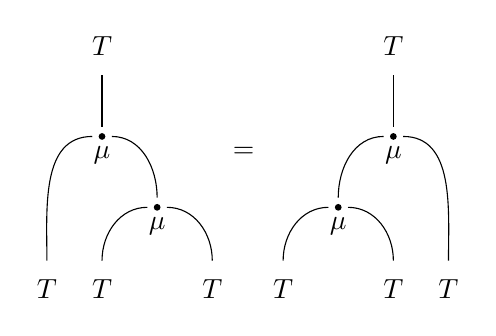
\begin{tikzpicture}
\def\delta{0.7}
\def\xa{0};
\def\xb{\delta};
\def\xc{\delta * 2};
\def\xd{\delta * 3};

\def \ya{0.8};
\def \yb{1.7};
\def \yc{2.6};

\node(a) at (\xa, 0) {};
\node(b) at (\xb, \yb) {};
\node(c) at (\xc, \ya) {};
\node(d) at (\xb, \yc) {};
\node(e) at (\xb, 0) {};
\node(f) at (\xd, 0) {};
\filldraw[black] (b) circle (1 pt);
\filldraw[black] (c) circle (1 pt);
\node [below] at (b) {$\mu$};
\draw (a) to [out=90, in=180]  node[left] {}(b);
\draw (c) to [out=90, in=0]  node[right] {} (b);
\draw (b) -- node[right] {} (d);
\draw (e) to [out=90, in=180]  node[left] {}(c);
\draw (f) to [out=90, in=0]  node[right] {}(c);
\node [below] at (c) {$\mu$};
\node [below] at (a) {$T$};
\node [above] at (d) {$T$};
\node [below] at (e) {$T$};
\node [below] at (f) {$T$};

\def\xe{2.5}
\node at (\xe, 1.5) {$=$};

\def\off{3}
\def\xa{\off + \delta * 0};
\def\xb{\off + \delta * 1};
\def\xc{\off + \delta * 2};
\def\xd{\off + \delta * 3};

\node(a) at (\xa, 0) {};
\node(b) at (\xc, 0) {};
\node(c) at (\xd, 0) {};
\node(d) at (\xb, \ya) {};
\node(e) at (\xc, \yb) {};
\node(f) at (\xc, \yc) {};
\filldraw[black] (d) circle (1 pt);
\filldraw[black] (e) circle (1 pt);
\node [below] at (d) {$\mu$};
\draw (a) to [out=90, in=180]  node[left] {}(d);
\draw (b) to [out=90, in=0]  node[right] {} (d);
\draw (e) -- node[right] {} (f);
\draw (d) to [out=90, in=180]  node[left] {}(e);
\draw (c) to [out=90, in=0]  node[right] {}(e);
\node [below] at (e) {$\mu$};
\node [below] at (a) {$T$};
\node [below] at (b) {$T$};
\node [below] at (c) {$T$};
\node [above] at (f) {$T$};
\end{tikzpicture}
\]

\subsection{String diagrams for the adjunction}

As we discussed before, an adjunction is a relation between a pair of functors, $L \colon \mathcal{D} \to \mathcal{C}$ and $R \colon \mathcal{C} \to \mathcal{D}$. It can be defined by a pair of natural transformations, the unit $\eta$ and the counit $\varepsilon$, satisfying triangular identities.

The unit of the adjunction can be illustrated by a ``cup''-shaped diagram:

\[
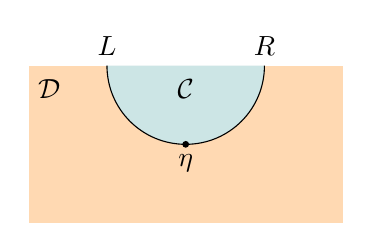
\begin{tikzpicture}

\def \xrightmost {2}
\def \xright         {1}
\def \xmid          {0}
\def \xleft           {-\xright}
\def \xleftmost   {-\xrightmost}

\def \ybot           {0}
\def \ymid          {1}
\def \ytop           {2}
\def \ylabel        {\ytop - 0.3}

% functor labels
\node [above] at (\xleft, \ytop)   {$L$};
\node [above] at (\xright, \ytop) {$R$};
% background
\filldraw[fill=orange!30, draw=white] (\xleftmost, \ytop) rectangle (\xrightmost, \ybot);
% cup
\draw [fill=blue!50!green!20] (\xleft, \ytop) to [out=-90, in=180] (\xmid, \ymid) to [out=0, in=-90] (\xright, \ytop);
% natural transformation
\filldraw [black] (\xmid, \ymid) circle (1 pt);
\node [below] at (\xmid, \ymid) {$\eta$};
% category labels
\node           at (\xmid, \ylabel)        {$\mathcal{C}$};
\node [right] at (\xleftmost, \ylabel) {$\mathcal{D}$};

\end{tikzpicture}
\]
The identity functor at the bottom of the diagram is omitted from the picture. The $\eta$ dot turns the identity functor below it to the composition $R \circ L$ above it.

Similarly, the counit can be visualized as a ``cap''-shaped string diagram with the implicit identity functor at the top:

\[
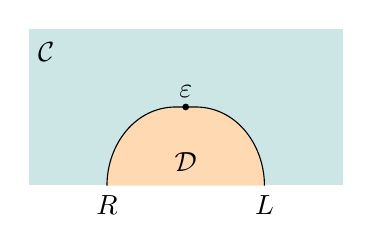
\begin{tikzpicture}
\def\xleft{0};
\def\xmid{1};
\def\xright{\xmid * 2};

\def \ybot{0};
\def \ymid{1};
\def \ytop{2 * \ymid};
\def \yt{2 * \ymid - 0.3};

\node [below] (a) at (\xleft, \ybot) {$R$};
\node(b) at (\xmid, \ymid) {};
\node[below] (c) at (\xright, \ybot) {$L$};

\filldraw[fill=blue!50!green!20, draw=white] (\xleft-1, \ytop) rectangle (\xright+1, \ybot);


\draw [fill=orange!30] (a.north) to [out=90, in=180] (b.west) -- (b.east) to [out=0, in=90] (c.north);

\filldraw[black] (b) circle (1 pt);
\node [above] at (b) {$\varepsilon$};

\node(l)[right] at (\xleft-1, \yt) {$\mathcal{C}$};
\node(r) at (\xmid, \ybot + 0.3) {$\mathcal{D}$};

\end{tikzpicture}
\]

Triangle identities can be easily expressed using string diagrams. They also make intuitive sense, as you can imagine pulling on the string from both sides to straighten the curve.

For instance, this is the first triangle identity. 

\[
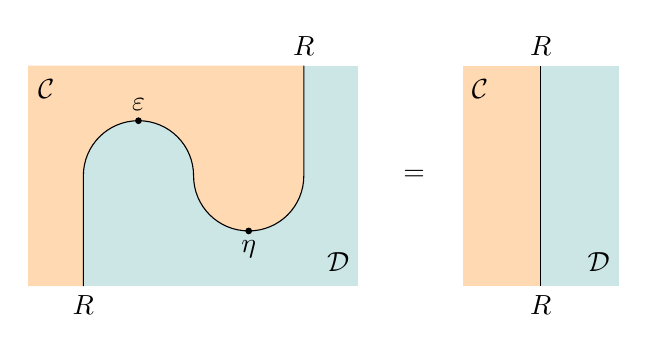
\begin{tikzpicture}
\def \dx {0.7}
\def \dy {0.7}

\def \xa{-3 * \dx};
\def \xb{-2 * \dx};
\def \xc{-1 * \dx};
\def \xd{0};
\def \xe{1 * \dx};
\def \xf{2 * \dx};
\def \xg{3 * \dx};

\def \ya{0};
\def \yb{1 * \dy};
\def \yc{2 * \dy};
\def \yd{3 * \dy};
\def \ye{4 * \dy};

\node [below] at (\xb, \ya) {$R$};
\node [right] at (\xd, \yc) {$L$};
\node [above] at (\xf, \ye) {$R$};
% background
\filldraw[fill=blue!50!green!20, draw=white] (\xa, \ye) rectangle (\xg, \ya);
% fill shape
\path [fill=orange!30] (\xa, \ya) to (\xb, \ya) to (\xb, \yc) to [out=90, in=180]  (\xc, \yd) to  [out=0, in=90] (\xd, \yc) to [out=-90, in=180] (\xe, \yb) to [out=0, in=-90] (\xf, \yc) to (\xf, \ye) to (\xa, \ye);

\draw (\xb, \ya) to (\xb, \yc) to [out=90, in=180]  (\xc, \yd) to  [out=0, in=90] (\xd, \yc) to [out=-90, in=180] (\xe, \yb) to [out=0, in=-90] (\xf, \yc) to (\xf, \ye);

\filldraw[black] (\xc, \yd) circle (1 pt);
\node [above] at (\xc, \yd) {$\varepsilon$};

\filldraw[black] (\xe, \yb) circle (1 pt);
\node [below] at (\xe, \yb) {$\eta$};

\node[right] at (\xa, \ye - 0.3) {$\mathcal{C}$};
\node[left] at (\xg, \ya + 0.3) {$\mathcal{D}$};

% right diagram

\node (eq) at (4 * \dy, \yc) {$=$};
\def \xh {6.3 * \dx}

\filldraw[fill=orange!30, draw=white] (\xh - 1, \ye) rectangle (\xh, \ya);
\filldraw[fill=blue!50!green!20, draw=white] (\xh, \ye) rectangle (\xh + 1, \ya);

\draw (\xh, \ye) -- (\xh, \ya);

\node[below] (bb) at (\xh, \ya) { $R$ };
\node[above] (bt) at (\xh, \ye) { $R$ };

\node(l)[right] at (\xh - 1, \ye - 0.3) {$\mathcal{C}$};
\node(r)[left] at (\xh + 1, \ya + 0.3) {$\mathcal{D}$};

\end{tikzpicture}
\]
Reading the left diagram bottom-to-top produces a series of mappings:

\[  Id_{\mathcal{D}} \circ R \xrightarrow{\eta \circ R} R \circ L \circ R \xrightarrow{R \circ \varepsilon} R \circ Id_{\mathcal{C}}  \]
This must be equal to the right-hand-side, which may be interpreted as the (invisible) identity natural transformation on $R$

\begin{exercise}
Draw the string diagrams for the second triangle identity.
\end{exercise}

\section{Monads from Adjunctions}

You might have noticed that the same symbol $\eta$ is used for the unit of the adjunction and for the unit of the monad. This is \emph{not} a coincidence. 

At first sight it might seem like we are comparing apples to oranges: an adjunction is defined with two functors between two categories and a monad is defined by one endofunctor operating on a single category. However, the composition of the two functors going in opposite directions is an endofunctor, and the unit of the adjunction maps the identity endofunctor to the endofunctor $R \circ L$. 

Compare this diagram:
\[
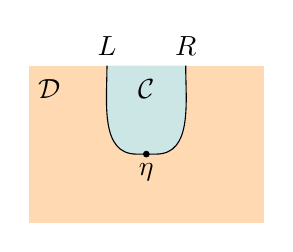
\begin{tikzpicture}
\def\xleft{0.5};
\def\xmid{1};
\def\xright{1.5};

\def \ybot{0};
\def \ymid{1};
\def \ytop{2 * \ymid};
\def \yt{2 * \ymid - 0.3};

\node [above] (a) at (\xleft, \ytop) {$L$};
\node(b) [below] at (\xmid, \ymid) {};
\node[above] (c) at (\xright, \ytop) {$R$};

\filldraw[fill=orange!30, draw=white] (\xleft-1, \ytop) rectangle (\xright+1, \ybot);


\draw [fill=blue!50!green!20] (a.south) to [out=-90, in=180] (b.west) -- (b.east) to [out=0, in=-90] (c.south);
\filldraw[black] (b) circle (1 pt);
\node [below] at (b) {$\eta$};

\node(l)[right] at (\xleft-1, \yt) {$\mathcal{D}$};
\node(r) at (\xmid, \yt) {$\mathcal{C}$};

\end{tikzpicture}
\]
with the one defining the monadic unit:

\[
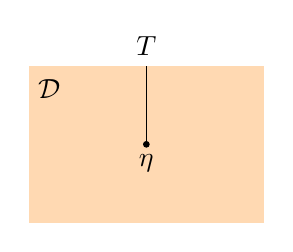
\begin{tikzpicture}
\def\xleft{0.5};
\def\xmid{1};
\def\xright{1.5};

\def \ybot{0};
\def \ymid{1};
\def \ytop{2 * \ymid};
\def \yt{2 * \ymid - 0.3};

\node(b) [above] at (\xmid, \ytop) {$T$};

\filldraw[fill=orange!30, draw=white] (\xleft-1, \ytop) rectangle (\xright+1, \ybot);

\draw (\xmid, \ymid) -- (\xmid, \ytop);

\filldraw[black] (\xmid, \ymid) circle (1 pt);
\node [below] at (\xmid, \ymid) {$\eta$};

\node(l)[right] at (\xleft-1, \yt) {$\mathcal{D}$};

\end{tikzpicture}
\]

It turns out that $T = R \circ L$ is in fact a monad, with the multiplication $\mu$ defined by the following diagram:

\[
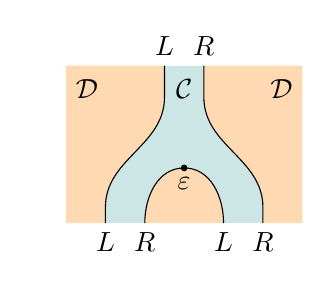
\begin{tikzpicture}
\def \xmid          {0};
\def \xr               {0.5};
\def \xrr             {1}
\def \xrm            {0.25}
\def \xrightmost {1.5}
\def \xl {-\xr}
\def \xll {-\xrr}
\def \xlm {-\xrm}
\def \xleftmost {-\xrightmost}

\def \ybot           {0};
\def \ymidbot     {0.20};
\def \yeps          {0.7};
\def \ymid          {1};
\def \ymidtop     {1.60}
\def \ytop           {2};
\def \ylabel        {\ytop - 0.3};
% functors
\node [above] at (\xlm, \ytop)  {$L$};
\node [above] at (\xrm, \ytop) {$R$};
\node [below] at (\xll, \ybot) {$L$};
\node [below] at (\xl, \ybot) {$R$};
\node [below] at (\xr, \ybot) {$L$};
\node [below] at (\xrr, \ybot) {$R$};

\filldraw[fill=blue!50!green!20, draw=white, draw=white] (\xleftmost, \ytop) rectangle (\xrightmost, \ybot);

% left area
\path [fill=orange!30] (\xleftmost, \ybot) to  (\xll, \ybot) to (\xll, \ymidbot) [out=90, in=-90] to (\xlm, \ymidtop) to  (\xlm, \ytop) to [out=180, in=180] (\xleftmost, \ytop);
% right area
\path [fill=orange!30] (\xrightmost, \ybot) to (\xrr, \ybot) to (\xrr, \ymidbot) [out=90, in=-90] to (\xrm, \ymidtop) to (\xrm, \ytop) to [out=0, in=180]  (\xrightmost, \ytop);
% cap
\draw [fill=orange!30] (\xl, \ybot) to [out=90, in=180] (\xmid, \yeps) to [out=0, in=90] (\xr, \ybot);
% left curve
\draw (\xll, \ybot) to (\xll, \ymidbot) [out=90, in=-90] to (\xlm, \ymidtop) to  (\xlm, \ytop);
% right curve
\draw (\xrr, \ybot) to (\xrr, \ymidbot) [out=90, in=-90] to (\xrm, \ymidtop) to (\xrm, \ytop);
% epsilon
\filldraw [black] (\xmid, \yeps) circle (1 pt);
\node [below] at (\xmid, \yeps) {$\varepsilon$};
% categories
\node [right] at (\xleftmost, \ylabel) {$\mathcal{D}$};
\node           at (\xmid, \ylabel)        {$\mathcal{C}$};
\node [left]   at (\xrightmost, \ylabel) {$\mathcal{D}$};

\end{tikzpicture}
\]
Reading this diagram bottom-up, we get the following transformation (imagine slicing it horizontally at the dot):
\[  R \circ L \circ R \circ L \xrightarrow{R \circ \varepsilon \circ L} R \circ L  \]
Compare this with the definition of monadic $\mu$:

\[
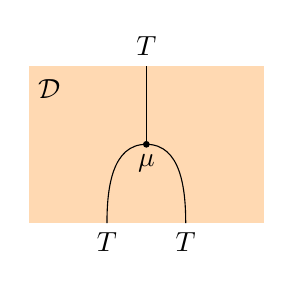
\begin{tikzpicture}
\def \xmid          {0};
\def \xr               {0.5};
\def \xrightmost {1.5};
\def \xl {-\xr};
\def \xleftmost {-\xrightmost};

\def \ybot           {0};
\def \ymid          {1};
\def \ytop           {2};
\def \ylabel        {\ytop - 0.3};

\node [above] at (\xmid, \ytop) {$T$};
\node [below] at (\xl, \ybot)      {$T$};
\node [below] at (\xr, \ybot)      {$T$};

\filldraw[fill=orange!30, draw=white] (\xleftmost, \ytop) rectangle (\xrightmost, \ybot);
% cap
\draw (\xl, \ybot) to [out=90, in=180] (\xmid, \ymid) to [out=0, in=90] (\xr, \ybot);
\draw (\xmid, \ymid) to (\xmid, \ytop);

\filldraw [black] (\xmid, \ymid) circle (1 pt);
\node [below] at (\xmid, \ymid) {$\mu$};

\node [right] at (\xleftmost, \ylabel) {$\mathcal{D}$};

\end{tikzpicture}
\]
This gives us the definition of $\mu$ for the monad $R \circ L$ as the double-whiskering of $\varepsilon$:
\[ \mu = R \circ \varepsilon \circ L \]

To complete the picture, we can use string diagrams to derive monadic laws using triangle identities. The trick is to replace all strings in monadic laws by pairs of parallel strings and then rearrange them according to the rules.

To summarize, every adjunction $L \dashv R$ with the unit $\eta$ and counit $\varepsilon$ defines a monad $(R \circ L, \eta, R \circ \varepsilon \circ L)$.

In the next chapter we'll see that, dually, the other composition, $L \circ R$ defines a comonad.

\begin{exercise}
Draw string diagrams to illustrate monadic laws (unit and associativity) for the monad derived from an adjunction.
\end{exercise}

\section{Examples of Monads from Adjunctions}

We'll go through several examples of adjunctions that generate some of the monads that we use in programming. Most examples involve functors that leave the category of Haskell types and functions, even though the round trip that generates the monad ends up being an endofunctor. This is why it's often impossible to express the adjunction in Haskell. 

To additionally complicate things, there is a lot of bookkeeping related to explicit naming of data constructors, which is necessary for type inference to work. This may sometimes obscure the simplicity on the underlying formulas.

\subsection{Free monoid and the list monad}
The list monad corresponds to the free monoid adjunction we've seen before. The unit of this adjunction, $\eta_X \colon X \to U (F X)$, injects the elements of the set $X$ as the generators of the free monoid. We represent the free monoid as a list, and its generators are singleton lists. This is exactly what we defined as the monadic unit:
\begin{haskell}
return x = [x]
\end{haskell}
To implement the counit, $\varepsilon_M \colon F (U M) \to M$, we take a monoid $M$, forget its multiplication, and use its set of elements as generators for the free monoid. The counit is a monoid morphism from that free monoid back to $M$. It turns out to be a special case of a catamorphism. 

Recall the Haskell implementation of a list catamorphism:
\begin{haskell}
foldMap :: Monoid m => (a -> m) -> ([a] -> m)
foldMap f = foldr mappend mempty . fmap f
\end{haskell}
The counit is just \hask{ foldMap id }, or 
\begin{haskell}
epsilon = foldr mappend mempty
\end{haskell}
Monad multiplication is given by the whiskering of the counit:
\[ \mu = U \circ \varepsilon \circ F \]
You can easily convince yourself that left whiskering doesn't do much here, since it's just a lifting of a monoid morphism by the forgetful functor. It just keeps the function while forgetting about it's special property of preserving structure. 

The right whiskering by $F$ is more interesting. It means taking the component of $\varepsilon$ at a free monoid generated from the set $X$. This  free monoid is defined by:
\begin{haskell}
mempty = []
mappend = (++)
\end{haskell}
which gives us the definition of $\mu$ or \hask{join}:
\begin{haskell}
join = foldr (++) []
\end{haskell}
As expected, this is the same as \hask{concat}.

\subsection{The currying adjunction and the state monad}

The state monad is generated by the adjunction between two functors that define the exponential object. The left functor is defined by a product with some fixed object $S$:
\[ L_S A = A \times S \]
We can implement it as a Haskell type:
\begin{haskell}
newtype L s a = L (a, s)
\end{haskell}
The right functor is the exponentiation, parameterized by the same object $S$:
\[ R_S C = C^S \]
In Haskell, it's a thinly encapsulated function type:
\begin{haskell}
newtype R s c = R (s -> c)
\end{haskell}

The monad is given by the composition of these two functors. On objects:
\[(R_S \circ L_S) A = (A \times S)^S \]
In Haskell we would write it as:
\begin{haskell}
newtype St s a = St (R s (L s a))
\end{haskell}
If you expand this definition, it's easy to recognize in it the \hask{State} functor:
\begin{haskell}
newtype State s a = State (s -> (a, s))
\end{haskell}

The unit of the adjunction $L_S \dashv R_S$ is:
\[ \eta_A \colon A \to (A \times S)^S \]
which can be implemented in Haskell as:
\begin{haskell}
eta :: a -> R s (L s a)
eta a = R (\s -> L (a, s))
\end{haskell}
You may recognized in it a thinly veiled version of \hask{return} for the state monad:
\begin{haskell}
return :: a -> State s a
return a = State (\s -> (a, s))
\end{haskell}

Here's the component of the counit of this adjunction at $C$:
\[ \varepsilon_C \colon C^S \times S \to C \]
It can be implemented in Haskell as:
\begin{haskell}
epsilon :: L s (R s a) -> a
epsilon (L ((R f), s))= f s
\end{haskell}
which, after stripping data constructors, is equivalent to \hask{apply}, or the uncurried version of \hask{runState}.

Monad multiplication $\mu$ is given by the whiskering of $\varepsilon$ from both sides:
\[ \mu = R_S \circ \varepsilon \circ L_S \]
This is how it translates to Haskell:
\begin{haskell}
mu :: R s (L s (R s (L s a))) -> R s (L s a)
mu = fmap epsilon
\end{haskell}
Here, whiskering on the right doesn't do anything other than select a component of the natural transformation. This is done automatically by Haskell's type inference engine. 

Whiskering on the left is done by lifting the component of the natural transformation. Again, type inference picks the correct implementation of \hask{fmap} (here, it's equivalent to precomposition) to perform that.

Compare this with the implementation of \hask{join}:
\begin{haskell}
join :: State s (State s a) -> State s a
join mma = State (fmap (uncurry runState) (runState mma))
\end{haskell}
Notice the dual use of \hask{runState}: 
\begin{haskell}
runState :: State s a -> s -> (a, s)
runState (State h) s = h s
\end{haskell}
When it's uncurried, its type signature becomes:
\begin{haskell}
uncurry runState :: (State s a , s) -> (a, s)
\end{haskell}
which is equivalent to that of \hask{epsilon}. When partially applied, it just strips the data constructor exposing the underlying function type:
\begin{haskell}
runState st ::  s -> (a, s)
\end{haskell}



\subsection{M-sets and the writer monad}

The writer monad:
\begin{haskell}
newtype Writer m a = Writer (a, m)
\end{haskell}
is parameterized by a monoid \hask{m}. This monoid is used for accumulating log entries. The adjunction we are going to use involves a category of M-sets for that monoid. 

An M-set is a set $S$ on which we define the action of a monoid $M$. Such an action is a mapping:
\[a \colon M \times S \to S \]
We often use the curried version of the action, with the monoid element in the subscript position. Thus $a_m$ becomes a function $S \to S$. 

This mapping has to satisfy some constraints. The action of the monoidal unit $1$ must not change the set, so it has to be the identity function:
\[ a_1 = id_S \]
and two consecutive actions must combine to an action of their monoidal product:
\[ a_{m_1} \circ a_{m_2} = a_{m_1 \cdot m_2} \]
This choice of the order of multiplication defines what it called the \emph{left action}. (The right action has the two monoidal elements swapped on the right-hand side.)

M-sets form a category $\mathbf{MSet}$. The objects are pairs $(S, a\colon M\times S \to S)$ and the arrows are  \emph{equivariant maps}, that is  functions between sets that preserve actions. 

A function $f \colon S \to R$ is an \emph{equivariant} mapping from $(S, a)$ to $(R, b)$ if the following diagram commutes, for every $m \in M$:

\[
 \begin{tikzcd}
 S 
 \arrow[r, "f"]
 \arrow[d, "a_m"]
 & R
\arrow[d, "b_m"]
 \\
S
 \arrow[r, "f"]
 & R
  \end{tikzcd}
\]
In other words, it doesn't matter if we first do the action $a_m$, and then map the set; or first map the set, and then do the corresponding action $b_m$.

There is a forgetful functor $U$ from $\mathbf{MSet}$ to $\mathbf{Set}$, which assigns the set $S$ to to the pair $(S, a)$, thus forgetting the action.  

Corresponding to it, there is a free functor $F$. Its action on a set $S$ produces an M-set that is a cartesian product of $S$ and $M$ (where $M$ is treated as a set of elements). An element of this M-set is a pair $(x \in S, m \in M)$ and the free action is defined by:
\[ \phi_n \colon (x, m) \mapsto (x, n \cdot m) \]

To show that $F$ is left adjoint to $U$ we have to construct a natural isomorphism, for any set $S$ and any M-set $Q$:
\[ \mathbf{MSet}( F S, Q) \cong \mathbf{Set}(S, U Q) \]
The trick here is to notice that an equivariant mapping on the left is fully determined by its action on the elements of the form $(x, 1)$.

The unit of this adjunction $\eta_S \colon S \to U (F S)$ maps an element $x$ to a pair $(x, 1)$. Compare this with the definition of \hask{return} for the writer monad:
\begin{haskell}
return a = Writer (a, mempty)
\end{haskell}

The counit is given by an equivariant map:
\[ \varepsilon_Q \colon F (U Q) \to Q \]

The left hand side is an M-set constructed by taking the underlying set of $Q$ and crossing it with $M$. The original action of $Q$ is forgotten and replaced by the free action. The obvious choice for counit is:
\[ \varepsilon_Q \colon (x, m) \mapsto a_m x \]
where $a$ is the action defined in $Q$.

Monad multiplication $\mu$ is given by the whiskering of the counit.
\[ \mu = U \circ \varepsilon \circ F \]
It means replacing $Q$ in the definition of $\varepsilon_Q$ with a free M-set whose action is the free action. (Whiskering with $U$ doesn't change anything.)
\[ \mu_S \colon ((x, m), n) \mapsto \phi_n (x, m) = (x, n \cdot m) \]
Compare this with the definition of \hask{join} for the writer monad:
\begin{haskell}
join :: Monoid m => Writer m (Writer m a) -> Writer m a
join (Writer ( Writer (x, m), m')) = Writer (x, mappend m' m)
\end{haskell}

\subsection{Pointed objects and the \hask{Maybe} monad}

Pointed objects are objects with a designated element. Since picking an element is done using the arrow from the terminal object, the category of pointed objects is defined using pairs $(A, p \colon 1 \to A)$, where $A$ is an object in $\mathcal{C}$. 

The arrows between these pairs are the arrows in $\mathcal{C}$ that preserve the points. Thus an arrow from $(A, p \colon 1 \to A)$ to $(B, q \colon 1 \to B)$ is an arrow $f \colon A \to B$ such that $q = f \circ p$. This category is also called a \emph{coslice category} and is written as $1/\mathcal{C}$.

There is an obvious forgetful functor $U \colon 1/\mathcal{C} \to \mathcal{C}$ that forgets the point. Its left adjoint is a free functor $F$ that maps an object $A$ to a pair $(1 + A, \text{Left})$. In other words, $F$ freely ads a point to an object. 

\begin{exercise}
Show that $U \circ F$ is the \hask{Maybe} monad.
\end{exercise}

The \hask{Either} monad is similarly constructed by replacing $1$ with a fixed object $E$.

\subsection{The continuation monad}

The continuation monad is defined in terms of a pair of contravariant functors in the category of sets. We don't have to modify the definition of an adjunction to work with contravariant functors. It's enough to select the opposite category for one of the endpoints. 

We'll define the left functor as:
\[ L_R \colon \mathbf{Set}^{op} \to \mathbf{Set} \] 
It maps a set $X$ to the hom-set in $\mathbf{Set}$:
\[ L_R X = \mathbf{Set}(X, R) \] 
This functor is parameterized by another set $R$. The right functor is defined by essentially the same formula:
\[ L_R \colon \mathbf{Set} \to \mathbf{Set}^{op} \] 
\[ L_R X = \mathbf{Set^{op}}(R, X)  = \mathbf{Set}(X, R) \] 


The composition $R \circ L$ can be written in Haskell as \hask{((x -> r) -> r)}, which is the same as the (covariant) endofunctor that defines the continuation monad.

\section{Monad Transformers}

Suppose that you want to combine multiple effects, say, state with the possibility of failure. One option is to define your own monad from scratch. You define a functor:
\begin{haskell}
newtype MaybeState s a = MS (s -> Maybe (a, s))
  deriving Functor
\end{haskell}
and the function to extract the result (or admit failure):
\begin{haskell}
runMaybeState :: MaybeState s a -> s -> Maybe (a, s)
runMaybeState (MS h) s = h s
\end{haskell}
You define the monad instance for it:
\begin{haskell}
instance Monad (MaybeState s) where
  return a = MS (\s -> Just (a, s))
  ms >>= k = MS (\s -> case runMaybeState ms s of
                       Nothing -> Nothing
                       Just (a, s') -> runMaybeState (k a) s')
\end{haskell}
and, if you are diligent enough, check that it satisfies the monad laws.

There is no general recipe for combining monads. In that sense, monads are not composable. However, we know that adjunctions are composable. We've seen how to get monads from adjunctions and, as we'll soon see, every monad can be obtained this way. So, if we can match the right adjunctions, the monads they generate will automatically compose.

Consider two composable adjunctions:
\[
 \begin{tikzcd}
  \mathcal{C}
  \arrow[rr, bend right, "R'"']
  &&
  \mathcal{D}
  \arrow[ll, bend right, "L'"']
    \arrow[rr, bend right, "R"']
&&
  \mathcal{E}
  \arrow[ll, bend right, "L"']
 \end{tikzcd}
\]
There are three monads in this picture. There is the inner monad $R' \circ L'$ and the outer monad $R \circ L$ as well as the composite $R \circ R' \circ L' \circ L$. 

If we call the inner monad $T = R' \circ L'$, then $R \circ T \circ L$ is the composite monad called the \emph{monad transformer}, because it transforms the monad $T$ into a new monad. 

In our example, \hask{Maybe} is the inner monad:
\[ T A = 1 + A \]
It is transformed using the outer adjunction $L_S \dashv R_S$, where:
\[ L_S A = A \times S \]
\[ R_S C = C^S \]
The result is:
\[ (1 + A \times S)^S\]
or, in Haskell:
\begin{haskell}
s -> Maybe (a, s)
\end{haskell}

In general, the inner monad $T$ is defined by its unit $\eta^i$ and multiplication $\mu^i$. The outer adjunction is defined by its unit $\eta^o$ and counit $\varepsilon^o$. 

The unit of the composite monad is the natural transformation:
\[ \eta \colon Id \to R \circ T \circ L \]
given by the string diagram:
\[
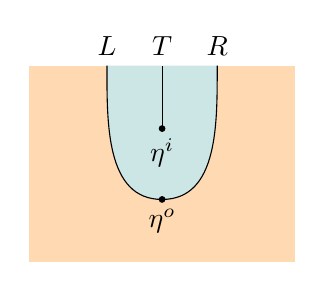
\begin{tikzpicture}
\def\xright{0.7};
\def\xleft{-\xright};
\def\xmid{0};

\def \ybot{0};
\def \ymid{0.8};
\def \yup{1.7};
\def \ytop{2.5};

\node [above] at (\xleft, \ytop) {$L$};
\node [above] at (\xmid, \ytop) {$T$};
\node [above] at (\xright, \ytop) {$R$};

\filldraw[fill=orange!30, draw=white] (\xleft-1, \ytop) rectangle (\xright+1, \ybot);

\draw [fill=blue!50!green!20] (\xleft, \ytop) to [out=-90, in=180] (\xmid, \ymid) to [out=0, in=-90] (\xright, \ytop);

\filldraw[black] (\xmid, \ymid) circle (1 pt);
\node [below] at (\xmid, \ymid) {$\eta^o$};
\filldraw[black] (\xmid, \yup) circle (1 pt);
\node [below] at (\xmid, \yup) {$\eta^i$};
\draw (\xmid, \yup) -- (\xmid,\ytop);

\end{tikzpicture}
\]
It is the vertical composition of the whiskered inner unit $R \circ \eta^i \circ L$ and the outer unit $\eta^o$. In components:
\[ \eta_A = R(\eta^i_{L A}) \circ \eta^o_A\]

The multiplication of the composite monad is a natural transformation:
\[ \mu \colon R \circ T \circ L \circ R \circ T \circ L \to R \circ T \circ L \]
given by the string diagram:

\[
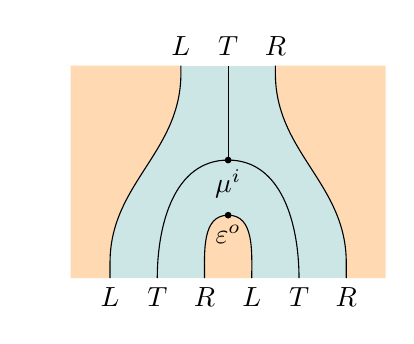
\begin{tikzpicture}
\def \xmid          {0};
\def \xr               {0.3};
\def \xrt             {0.9};
\def \xrr             {1.5}
\def \xrm            {0.6}
\def \xrightmost {2}
\def \xl {-\xr}
\def \xlt {-\xrt}
\def \xll {-\xrr}
\def \xlm {-\xrm}
\def \xleftmost {-\xrightmost}

\def \ybot           {0};
\def \ymidbot     {0.2};
\def \yeps          {0.8};
\def \ymu           {1.5}; % mu
\def \ymid          {1.9};
\def \ymidtop     {2.6}
\def \ytop           {2.7};
\def \ylabel        {\ytop - 0.3};
% functors
\node [above] at (\xlm, \ytop)  {$L$};
\node [above] at (\xmid, \ytop)  {$T$};
\node [above] at (\xrm, \ytop) {$R$};

\node [below] at (\xll, \ybot) {$L$};
\node [below] at (\xlt, \ybot) {$T$};
\node [below] at (\xl, \ybot) {$R$};
\node [below] at (\xr, \ybot) {$L$};
\node [below] at (\xrt, \ybot) {$T$};
\node [below] at (\xrr, \ybot) {$R$};

\filldraw[fill=blue!50!green!20, draw=white, draw=white] (\xleftmost, \ytop) rectangle (\xrightmost, \ybot);

% left area
\path [fill=orange!30] (\xleftmost, \ybot) to  (\xll, \ybot) to (\xll, \ymidbot) [out=90, in=-90] to (\xlm, \ymidtop) to  (\xlm, \ytop) to [out=180, in=180] (\xleftmost, \ytop);
% right area
\path [fill=orange!30] (\xrightmost, \ybot) to (\xrr, \ybot) to (\xrr, \ymidbot) [out=90, in=-90] to (\xrm, \ymidtop) to (\xrm, \ytop) to [out=0, in=180]  (\xrightmost, \ytop);
% cap
\draw [fill=orange!30] (\xl, \ybot) to [out=90, in=180] (\xmid, \yeps) to [out=0, in=90] (\xr, \ybot);
% fork
\draw (\xlt, \ybot) to [out=90, in=180] (\xmid, \ymu) to [out=0, in=90] (\xrt, \ybot);

% left curve
\draw (\xll, \ybot) to (\xll, \ymidbot) [out=90, in=-90] to (\xlm, \ymidtop) to  (\xlm, \ytop);
% right curve
\draw (\xrr, \ybot) to (\xrr, \ymidbot) [out=90, in=-90] to (\xrm, \ymidtop) to (\xrm, \ytop);
% epsilon
\filldraw [black] (\xmid, \yeps) circle (1 pt);
\node [below] at (\xmid, \yeps) {$\varepsilon^o$};

% mu
\filldraw [black] (\xmid, \ymu) circle (1 pt);
\node [below] at (\xmid, \ymu) {$\mu^i$};
\draw (\xmid, \ymu) -- (\xmid, \ytop);

\end{tikzpicture}
\]
It's the vertical composition of the multiply whiskered outer counit:
\[ R \circ T \circ L \circ \varepsilon^o \circ R \circ T \circ L \]
followed by the whiskered inner multiplication $R \circ \mu^i \circ L$. In components:
\[ \mu_C = R(\mu^i_{L C}) \circ (R \circ T) (\varepsilon^o_{(T\circ L)C})\]

Let's unpack these equations for the case of the state monad transformer. Here, the left functor is the product functor \hask{(a, s)} and the right functor is the exponential, a.k.a., the reader functor \hask{s->a}. 

and the counit $\varepsilon^o_Y$ is function application, for the function \hask{f :: x -> y}:
\begin{haskell}
epsilon (f, x) = f x
\end{haskell}
We'll keep the inner monad $(T, \eta^i, \mu^i)$ arbitrary. In Haskell, we'll call these \hask{m}, \hask{return}, and \hask{join}.

The monad that we get by applying the monad transformer for the state monad to the monad $T$, is the composition $R \circ T \circ L$ or, in Haskell:
\begin{haskell}
newtype StateT s m a = StateT (s -> m (a, s))
\end{haskell}

\begin{haskell}
runStateT :: StateT s m a -> s -> m (a, s)
runStateT (StateT h) s = h s
\end{haskell}

The unit of the monad transformer is the composition:
\[ \eta_A = R(\eta^i_{L A}) \circ \eta^o_A \]

There are a lot of moving parts in this formula, so let's analyze it step-by-step. We start from the right: we have the $A$-component of the unit of the adjunction. It's an arrow from $A$ to $R (L A)$. It's tranlated to a Haskell function. If we apply this function to a variable \hask{x :: a}, we can pass the result to the next function in chain, which is $R(\eta^i_{L A})$.

Recall that the unit of the currying adjunction $\eta^o_A$ is defined by:
\begin{haskell}
eta x = \s -> (x, s)
\end{haskell}
so the result is again a function whose type is \hask{s -> (a, s)}. Keep this in mind as we procede. 

Now, what is $R(\eta^i_{LA})$? It's the component of \hask{return} of the inner monad taken at $L A$. Here, $L A$ is the type \hask{(a, s)}. So we are instantiating \hask{return} as a function \hask{(a, s) -> m (a, s)}. (The type inferencer will do this automatically for us.)

Next, we are lifting this component of \hask{return} using $R$. Here, $R$ is the exponential $(-)^S$, so it lifts a function by post-composition. It will post-compose \hask{return} to whatever function is passed to it. That's exactly the function that we produced using \hask{eta}. Notice that the types match: we are post-composing \hask{(a, s) -> m (a, s)} after \hask{s -> (a, s)}. 

We can write the result of this composition as:
\begin{haskell}
return x = StateT (\s -> return (x, s))
\end{haskell}
with the data constructor \hask{StateT} to make the type checker happy. This is the \hask{return} of the composite monad in terms of the \hask{return} of the inner monad.

The same reasoning can be applied to the formula for the component of the composite $\mu$ at some $C$: 
\[ \mu_C = R(\mu^i_{L C}) \circ (R \circ T) (\varepsilon^o_{(T\circ L)C})\]
The inner $\mu^i$ is the \hask{join} of the monad \hask{m}. Applying $R$ turns it into post-composition. 

The outer $\varepsilon^o$ is function application taken at \hask{m (a, s)} which, inserting the appropriate data constructors, can be written as \hask{uncurry runStateT}:
\begin{haskell}
uncurry runStateT :: (StateT s m a, s) -> m (a, s)
\end{haskell}
The application of $(R \circ T)$ lifts this component of $\varepsilon$ using the composition of functors $R$ and $T$. The former is implemented as  post-composition, and the latter is the \hask{fmap} of the monad $m$. 

Putting all this together, we get a point-free formula for \hask{join} of the state monad transformer:
\begin{haskell}
join :: StateT s m (StateT s m a) -> StateT s m a
join mma = StateT (join . fmap (uncurry runStateT) . runStateT mma)
\end{haskell}
Here, the partially applied \hask{runStateT mma} strips off the data constructor from the argument \hask{mma}:
\begin{haskell}
runStateT mma :: s -> m (a, x)
\end{haskell}

Our earlier example of \hask{MaybeState} can now be rewritten using a monad transformer:
\begin{haskell}
type MaybeState s a = StateT s Maybe a
\end{haskell}

The original \hask{State} monad can be recovered by applying the \hask{StateT} monad transformer to the identity functor, which has a \hask{Monad} instance defined in the library (notice that the last type variable \hask{a} is skipped in this definition):
\begin{haskell}
type State s = StateT s Identity
\end{haskell}

Other monad transformers follow the same pattern. They are defined in the Monad Transformer Library, \hask{MTL}.

\section{Monad Algebras}

Every adjunction generates a monad, and so far we've been able to define adjunctions for all the monads of interest for us. But is every monad generated by an adjunction? The answer is yes, and there are usually many adjunctions---in fact a whole category of adjunctions---for every monad.

Finding an adjunction for a monad is analogous to factorization. We want to express a functor as a composition of two other functors. The problem is complicated by the fact that this factorization also requires finding an appropriate intermediate category. We'll find such a category by studying algebras for a monad.

A monad is defined by an endofunctor, so it's possible to define algebras for this endofunctor. Mathematicians often think of monads as tools for generating expressions and algebras as tools for evaluating those expressions. However, expressions generated by monads impose some compatibility conditions on those algebras. 

Consider the earlier example of the expression monad \hask{Ex}. An algebra for this monad is a choice of the carrier type, say \hask{Char} and an arrow
\begin{haskell}
alg :: Ex Char -> Char
\end{haskell}
Since \hask{Ex} is a monad, it defines a unit, or \hask{return}, which is a polymorphic function that can be used to generate simple expressions from values. The unit of \hask{Ex} is:
\begin{haskell}
return x = Var x
\end{haskell}
We can instantiate the unit for an arbitrary type, in particular for the carrier type of our algebra. It makes sense that evaluating \hask{Var c}, where \hask{c} is an element of \hask{Char} should give us back the same \hask{c}. In other words, we'd like:
\begin{haskell}
 alg . return = id
\end{haskell}
This condition immediately eliminates a lot of algebras, such as:
\begin{haskell}
alg (Var c) = 'a' -- not compatible with the monad Ex
\end{haskell}

The second condition we'd like to impose is that the algebra respects substitution. A monad lets us flatten nested expressions using \hask{join}. An algebra lets us evaluate such expressions. 

There are two ways of doing that: we can apply the algebra to a flattened expression, or we can apply it to the inner expression first (using \hask{fmap}), and then evaluate the resulting expression. 
\begin{haskell}
 alg (join mma) = alg (fmap alg mma)
\end{haskell}
where \hask{mma} is of the type \hask{Ex (Ex Char)}.

In category theory these two conditions define a monad algebra. 

$(A, \alpha \colon T A \to A)$ is a \emph{monad algebra} for the monad $(T, \mu, \eta)$ if the following diagrams commute:
\[
 \begin{tikzcd}
 A
 \arrow[r, "\eta_A"]
 \arrow[dr, "id_A"']
 & T A
 \arrow[d, red, "\alpha"]
 \\
 & A
 \end{tikzcd}
  \hspace{30pt}
 \begin{tikzcd}
T(T A) 
\arrow[r, red, "T \alpha "]
\arrow[d, "\mu_A"]
&TA
\arrow[d, red, "\alpha"]
\\
T A
\arrow[r, red, "\alpha"]
& A
 \end{tikzcd}
\]

Since monad algebras are just special kinds of algebras, they form a sub-category of algebras. Recall that algebra morphisms are arrows that satisfy the following condition:
\[
 \begin{tikzcd}
 T A 
 \arrow[r, "T f"]
 \arrow[d, "\alpha"]
 & T B
\arrow[d, "\beta"]
 \\
 A
 \arrow[r, "f"]
 & B
  \end{tikzcd}
\]
These laws are sometimes called the unit law and the multiplication law for monad algebras.

In light of this definition, we can re-interpret the second monad-algebra diagram as asserting that the structure map of a monad algebra is also an algebra morphism from $(T A, \mu_A)$ to $(A, \alpha)$. This will come in handy in what follows.

\subsection{Eilenberg-Moore category}

The category of monad algebras for a given monad $T$ on $ \mathcal{C}$ is called the Eilenberg-Moore category and is denoted by $ \mathcal{C}^T$. 

There is an obvious forgetful functor $U^T$ from $ \mathcal{C}^T$ to $ \mathcal{C}$. It maps an algebra $(A, \alpha)$ to its carrier $A$, and treats algebra morphisms as regular morphisms between carriers. 

There is a free functor $F^T$ that is left adjoint to $U^T$. It's defined to map an object $A$ of $ \mathcal{C}$ to a monad algebra with the carrier $T A$. The structure map of this algebra is the component of monad multiplication $\mu_A \colon T(TA) \to TA$. 

It's easy to check that $(T A, \mu_A)$ is indeed a monad algebra---the commuting conditions follow from monad laws. Indeed, substituting the algebra $(T A, \mu_A)$ into the monad-algebra diagrams, we get (with the algebra part drawn in red):
\[
 \begin{tikzcd}
 T A
 \arrow[r, "\eta_{TA}"]
 \arrow[dr, "id_{TA}"']
 & T(T A)
 \arrow[d, red, "\mu_A"]
 \\
 & T A
 \end{tikzcd}
  \hspace{30pt}
 \begin{tikzcd}
T(T(T A))
\arrow[r, red, "T \mu_A "]
\arrow[d, "\mu_{TA}"]
&T(TA)
\arrow[d, red, "\mu_A"]
\\
T (T A)
\arrow[r, red, "\mu_A"]
& T A
 \end{tikzcd}
\]
The first diagram is just the left monadic unit law in components. The $\eta_{T A}$ arrow corresponds to the whiskering of $\eta \circ T$. The second diagram is the associativity of $\mu$ with the two whiskerings $\mu \circ T$ and $T \circ \mu$ expressed in components.

As is true for all adjunctions, the composition $U^T \circ F^T$ is a monad. However this particular monad is identical to the original monad $T$. 

Indeed, on objects, it first maps $A$ to a free monad algebra $(T A, \mu)$ and then forgets about the structure map. The net result is the mapping of $A$ to $T A$, which is exactly what the original monad did. On arrows, it lifts an arrow $f \colon A \to B$ using $T$. The fact that the arrow $T f$ is an algebra morphism from $(T A, \mu_A)$ to $(T B, \mu_B)$ follows from naturality of $\mu$:
\[
 \begin{tikzcd}
 T (T A)
 \arrow[r, "T( T f)"]
 \arrow[d, "\mu_A"]
 & T (T B)
\arrow[d, "\mu_B"]
 \\
 T A
 \arrow[r, "T f"]
 & T B
  \end{tikzcd}
\]



To prove that we have an adjunction, we can either construct the natural isomorphism between hom-sets, or define two natural transformations to serve as the unit and the counit of the adjunction. 

We define the unit of the adjunction as the monadic unit $\eta$ of $T$. The counit is a natural transformation whose component at $(A, \alpha)$ is an algebra morphism from the free algebra generated by $A$, that is $(T A, \mu_A)$, back to $(A, \alpha)$. As we've seen earlier, $\alpha$ itself is such a morphism. We can therefore pick $\varepsilon_{(A, \alpha)} = \alpha$.

Triangular identities for these definitions of $\eta$ and $\varepsilon$ follow from unit laws for the monad and the monad algebra.

The whiskering of $U^T \circ \varepsilon F^T$ in components means instantiating $\varepsilon$ at $(T A, \mu_A)$, which produces $\mu_A$ (the action of $U^T$ on arrows is trivial). 

We have thus shown that for any monad $T$ we can define the Eilenberg-Moore category and a pair of adjoint functors that give rise to this monad.

\subsection{Kleisli category}

Inside every Eilenberg-Moore category there is a smaller Kleisli category struggling to get out. This smaller category is the image of the free functor we have constructed in the previous section. 

Despite appearances, the image of a functor does not necessarily define a subcategory. Granted, it maps identities to identities and composition to composition. The problem may arise if two arrows that were not composable in the source category become composable in the target category. This may happen if the target of the first arrow is mapped to the same object as the source of the second arrow. However, the free functor $F^T$ maps distinct objects into distinct free algebras, so its image is indeed a subcategory of $\mathcal{C}^T$.

We have encountered the Kleisli category before. There are many ways of constructing the same category, and the simplest way to describe the Kleisli category is in terms of Kleisli arrows. 

A Kleisli category for the monad $(T, \eta, \mu)$ is denoted by $\mathcal{C}_T$. Its objects are the same as the objects of $\mathcal{C}$, but an arrow in $\mathcal{C}_T$ from $A$ to $B$ is represented by an arrow in $\mathcal{C}$ that goes from $A$ to $T B$. You may recognize it as the Kleisli arrow \hask{ a -> m b} we've defined before. Because $T$ is a monad, these Kleisli arrows can be composed using the ``fish'' operator \hask{<=<}. 

To establish the adjunction, let's define the left functor $L_T \colon \mathcal{C} \to \mathcal{C}_T$ as identity on objects. We still have to define what it does to arrows. It must map a regular arrow $f \colon A \to B$ to a Kleisli arrow from $A$ to $B$. This Kleisli arrow is represented by an arrow $A \to T B$ in $\mathcal{C}$. We pick the composite $\eta_B \circ f$:
\[ L_T f \colon A \xrightarrow{f} B \xrightarrow{\eta_B} T B\]

The right functor $R_T \colon \mathcal{C}_T \to \mathcal{C}$ is defined on objects as a mapping that takes an $A$ in the Kleisli category to an object $T A$ in $\mathcal{C}$. Given a Kleisli arrow from $A$ to $B$, which is represented by an arrow $g \colon A \to T B$, $R_T$ will map it to an arrow $R_T A \to R_T B$, that is an arrow $T A \to T B$ in $\mathcal{C}$. We take this arrow to be $\mu_B \circ T g$:
\[  T A \xrightarrow{T g} T(T B) \xrightarrow{\mu_B} T B\]

To establish the adjunction, we show the isomorphism of hom-sets:
\[\mathcal{C}_T(L_T A, B) \cong \mathcal{C}(A, R_T B)\]
An element of the left hand-side is a Kleisli arrow, which is represented by $f \colon A \to T B$. We can find the same arrow on the right hand side, since $R_T B$ is $T B$. So the isomorphism is between Kleisli arrows in $\mathcal{C}^T$ and the arrows in $\mathcal{C}$ that represent them.

The composite $R_T \circ L_T$ is equal to $T$ and, indeed, it can be shown that this adjunction generates the original monad. 

In general, there may be many adjunctions that generate the same monad. Adjunctions themselves form a 2-category, so it's possible to compare adjunctions using adjunction morphisms (1-cells in the 2-category). It turns out that the Kleisli adjunction is the initial object among all adjunctions that generate a given monad. Dually, the Eilenberg-Moore adjunction is terminal. 

\section{Monoidal Functors}


\subsection{notes}


\begin{exercise}
\end{exercise}

\begin{haskell}
\end{haskell}

\[
 \begin{tikzcd}
  \end{tikzcd}
\]

\[   \mathbf{Set} \]
\[   \mathcal{C} \]

\end{document}